%% 文献阅读笔记

\documentclass[manual, oneside]{whuthesis}
\usepackage{amsfonts,amssymb}

\setcounter{tocdepth}{2}
\setcounter{secnumdepth}{3}

\begin{document}
%----------- 封面部分 ----------- %%
\stunum{20171004186}
\title{典型的分类网络}
\school{计算机学院}
\major{空间信息与数字技术}
\author{吴朝明}
\advisor{xxx}
\proftitle{教授}
\maketitlepage            % 封面
\makestatement            % 申明

%%----------- 前言部分 ----------- %%
% % 中英文摘要

\begin{cnabstract}{关键词 1, 关键词 2, 关键词 3}
  请使用英文逗号分割关键词!

  摘要内容摘要内容摘要内容摘要内容摘要内容摘要内容摘要内容摘要内容摘要内容摘要内容摘要内容摘要内容摘要内容摘要内容

  摘要内容应概括地反映出本论文的主要内容,主要说明本论文的研究目的、内容、方法、成果和结论。要突出本论文的创造性成果或新见解,不要与引言相混淆。语言力求精练、准确。在摘要的下方另起一行,注明本文的关键词(3--5 个)。摘要与关键词应在同一页。
\end{cnabstract}


\begin{enabstract}{Key1, Key2, Key3}
  Please use comma to separate key words!

  This is abstract. This is abstract. This is abstract. This is abstract. This is abstract. This is abstract. This is abstract. This is abstract.

  The content of English abstract is the same as Chinese abstract. The last line is English keywords (3--5 keywords).
\end{enabstract}
  % 摘要
\newpage
\contents                 % 目录

%%----------- 主体部分 ----------- %%
% chapter2

\chapter{典型神经网络}

\section{AlexNet}
Alex Krizhevsky等人\cite{hinton2012imagenet}提出的,并由此网络模型获得了2012年的ImageNet ILSVRC的冠军。AlexNet采用5层卷积加3层全连接和一个softmax分类器的结构,使用两个GPU进行训练,最后在ImageNet数据集上取得了优秀的成绩。

ImageNet数据集有1500万张带标签的高分辨率图像,共有22000个类别。ILSVRC比赛使用ImageNet的子集,有1000个类别。在ImageNet数据集中,包含有各种分辨率的图像,AlexNet模型却需要一个恒定的输入维数,下采样这些图像得到固定的分辨率$256\times256$。

AlexNet整体结构比较简单,主要特点有:采用最大池化代替以往的平均池化,这是因为平均池化容易出现特征图模糊的现象;卷积层后采用Relu激活函数代替Sigmoid激活函数,用于缓解神经网络中的梯度消息问题;并且引入Dropout随机丢弃一部分神经元,防止训练过程中出现过拟合现象;反向传播过程中使用随机梯度下降算法用于优化网络训练过程,提高收敛速度。其网络结构如~\ref{fig:AlexNet_net}所示:
\begin{figure}[h!]
	\centering
	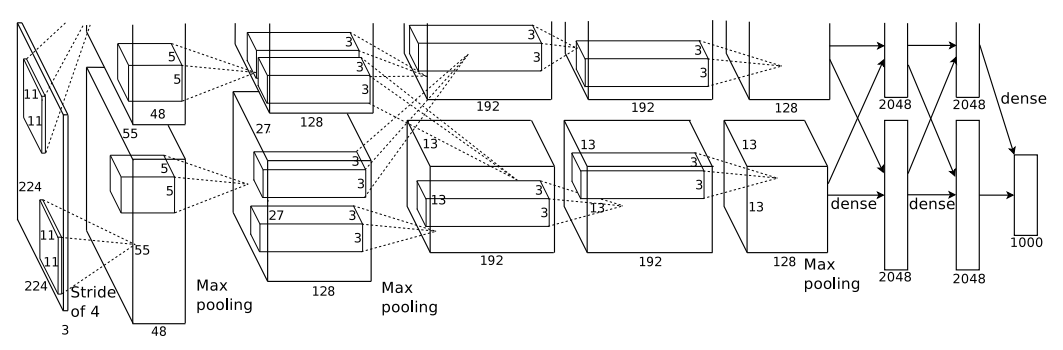
\includegraphics[width=\linewidth]{readings_figures/AlexNet_net.png}
	\caption{AlexNet网络结构}
	\label{fig:AlexNet_net}
\end{figure}

从图中可以看出,ALexNet包含有8层网络结构,其中前5层为卷积层,后3层为全连接层。作者将其在两个GPU上运行,卷积层中只有在第3层两个GPU中才有数据的交流,全连接层中两个GPU之间都有连接。相关的参数设置总结如下:
\begin{itemize}
	\item 卷积层1:输入$224\times224\times3$,卷积核$11\times11\times3$,卷积核个数96,步长4,padding为0,输出$96\times55\times55$;
	\item 池化层:$3\times3$,步长2,最大池化,输出$96\times27\times27$;
	\item 卷积层2:输入$96\times27\times27$,卷积核$5\times5$,卷积核个数256,步长1,padding为2,输出$256\times13\times13$;
	\item 池化层:$3\times3$,步长2,最大池化,输出$256\times13\times13$;
	\item 卷积层3:输入$256\times13\times13$,卷积核$3\times3$,卷积核个数384,步长1,padding为1,输出$384\times13\times13$;
	\item 卷积层4:输入$384\times13\times13$,卷积核$3\times3$,卷积核个数384,步长1,padding为1,输出$384\times13\times13$;
	\item 卷积层5:输入$384\times13\times13$,卷积核$3\times3$,卷积核个数256,步长1,padding为1,输出$256\times13\times13$;
	\item 池化层:$3\times3$,步长2,最大池化,输出$256\times6\times6$;
	\item 全连接层1:共4096个神经元;
	\item 全连接层2:共4096个神经元;
	\item 全连接层3:共1000个神经元;
\end{itemize}

\section{VGGNet}

Simonyan等人\cite{simonyan2014very}于2014年提出的VGG网络结构在当年的ILSVRC比赛中定位和分类分别获得了第一名和第二名的优秀成绩。VGGNet与AlexNet相似,都是由卷积层和全连接层构成,但VGGNet的性能以及使用程度都在AlexNet上有了较大的改进。在文章中,作者主要探索了卷积网络架构设计中网络深度对网络性能的影响,通过在网络层中使用非常小的$3\times3$的卷积滤波器,保证了在添加卷积层时能够稳定地增加网络深度。

在原文中,作者提出了多种深度的网络结构,如~\ref{fig:VGGNet_net}所示:
\begin{figure}[h!]
	\centering
	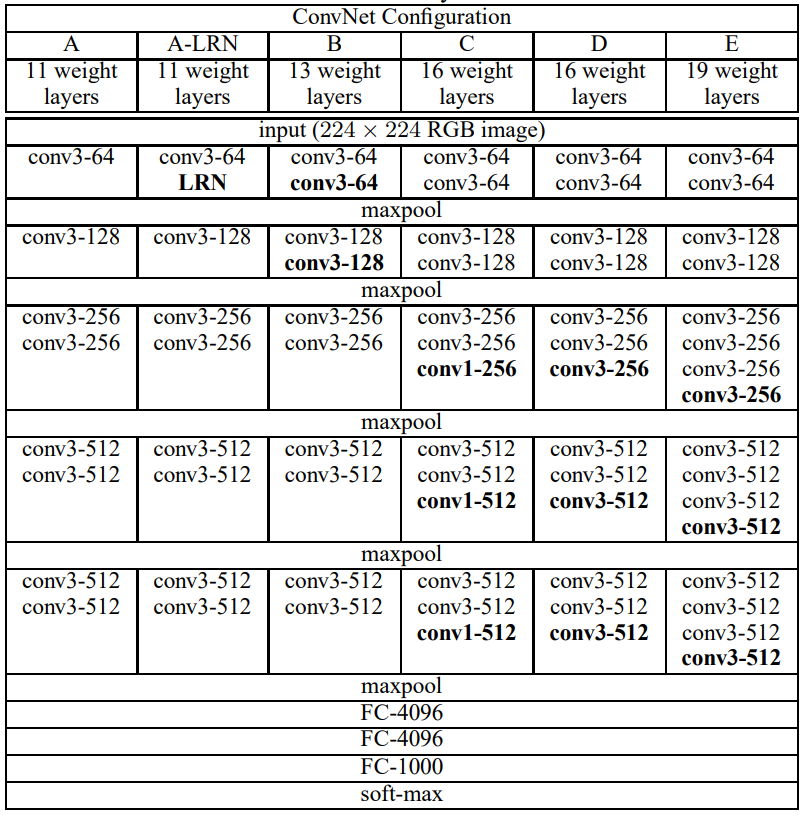
\includegraphics[width=\linewidth]{readings_figures/VGGNet_net.png}
	\caption{VGG网络结构}
	\label{fig:VGGNet_net}
\end{figure}

VGGNet由5层卷积层,3层全连接层和1层softmax输出层组成,5个卷积层的后面都接有最大池化层,激活函数采用ReLU函数。需要注意的是,在VGGNet网络结构中,并不是每一层卷积层后面都接有池化层。相较于AlexNet而言,VggNet采用了更小的卷积核,以及更多的卷积子层。VGGNet中卷积核大小全为$3\times3$,作者认为两个$3\times3$卷积核堆积有$5\times5$的有效感受野,三个这样的层则具有$7\times7$的有效感受野,这样的话结合了三个非线性修正层,使得决策函数更具有判别性,同时能够减少参数量。而在测试阶段,将3层全连接层改为卷积层,使得对测试时输入的图像尺寸没有要求。该文中通过多组实验对比说明了VGGNet在大部分数据上的性能较好,同时也证明了AlexNet中LRN操作对网络性能没有影响。


\section{GoogLeNet}

Szegedy等人\cite{szegedy2015going}提出的GoogLeNet(inception v1)在2014年的ILSVRC比赛中获得了第一名的成绩。相较于VGGNet继承了AlexNet网络结构并进行加深和使用小卷积核而言,GoogLeNet则是尝试了新的网络结构,尽管深度比AlexNet和VGGNet都更多,有22层,但参数只有500万个,比两者都要小得多,特点在于采用了Inception模块。

在以往,提升神经网络的性能最常见的方法就是提高网络深度(网络层次的数量)和宽度(神经元的数量),但这样也会出现很多问题。参数过多的话,训练集如果数量不够多就容易出现过拟合的情况;网络越深,宽度越大,计算量也会越大;网络越深,容易出现梯度弥散问题,难以优化模型。为此,Google团队提出了Inception网络结构。

Inception架构的主要想法在于如何近似卷积神经网络中的最优局部稀疏结构并用其他的密集组件进行覆盖。为此,首先提出了最初的基本结构~\ref{fig:GoogLeNet_Inception_module_naive}:

\begin{figure}[htbp]
	\centering
	\subfloat[Inception module naive version]{
		\centering
		\begin{minipage}{0.48\linewidth}
			\centering
			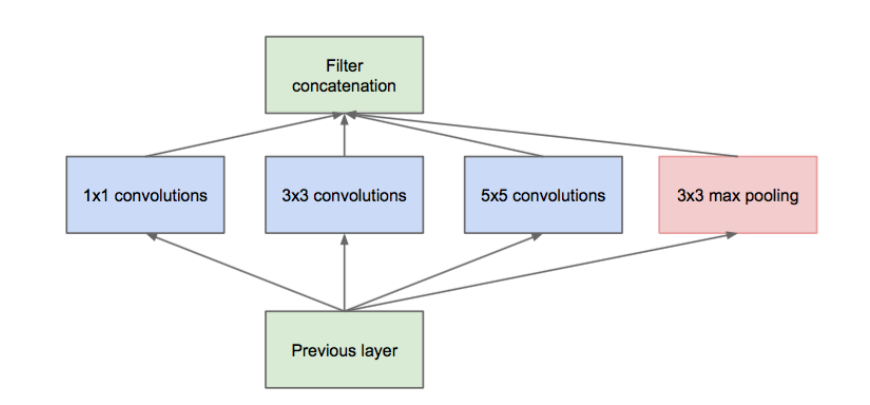
\includegraphics[width = \linewidth]{readings_figures/GoogLeNet_Inception_module_naive.png}
			\label{fig:GoogLeNet_Inception_module_naive}
		\end{minipage}
	}
	\centering
	\subfloat[Inception module with dimensionality reduction]{
		\centering
		\begin{minipage}{0.48\linewidth}
			\centering
			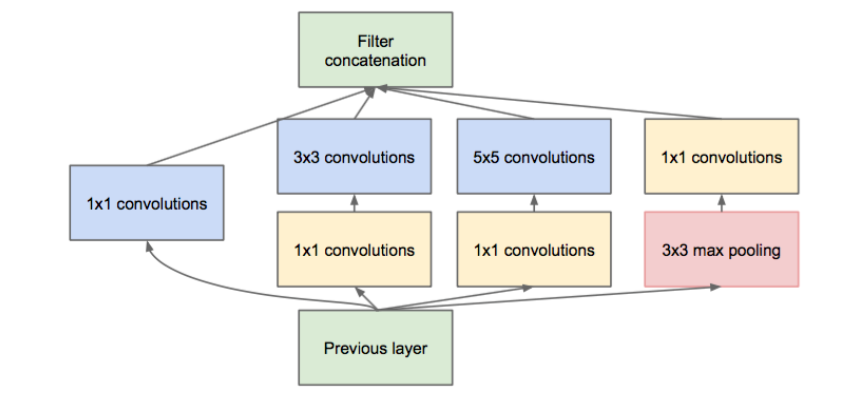
\includegraphics[width = \linewidth]{readings_figures/GoogLeNet_Inception_module_v1.png}
			\label{fig:GoogLeNet_Inception_module_v1}
		\end{minipage}
	}
	\centering
	\caption{GoogLeNet Inception架构}
	\label{fig:GoogLeNet_Inception}
\end{figure}

最初的Inception架构含有4个分支,前3个分支进行卷积之后得到的特征图大小是一致的,于是在进行卷积之后就可以堆叠起来作为下一层的输入。其中的卷积核大小分别为$1\times1$,$3\times3$,$5\times5$,这样的设置更多的是为了方便而并非是必须,第4个分支是池化操作。但是这种原始结构的缺点在于$5\times5$的卷积核计算量太大,为此,在$3\times3$,$5\times5$的卷积层前,$3\times3$的最大池化层后加上$1\times1$的卷积降维,即Inception v1的网络架构,如图~\ref{fig:GoogLeNet_Inception_module_v1},$1\times1$的卷积核的主要目的减小维度和修正线性激活。

GoogLeNet的具体网络结构如图~\ref{fig:GoogLeNet_net},网络的具体描述如下:

\begin{figure}[htbp]
	\centering
	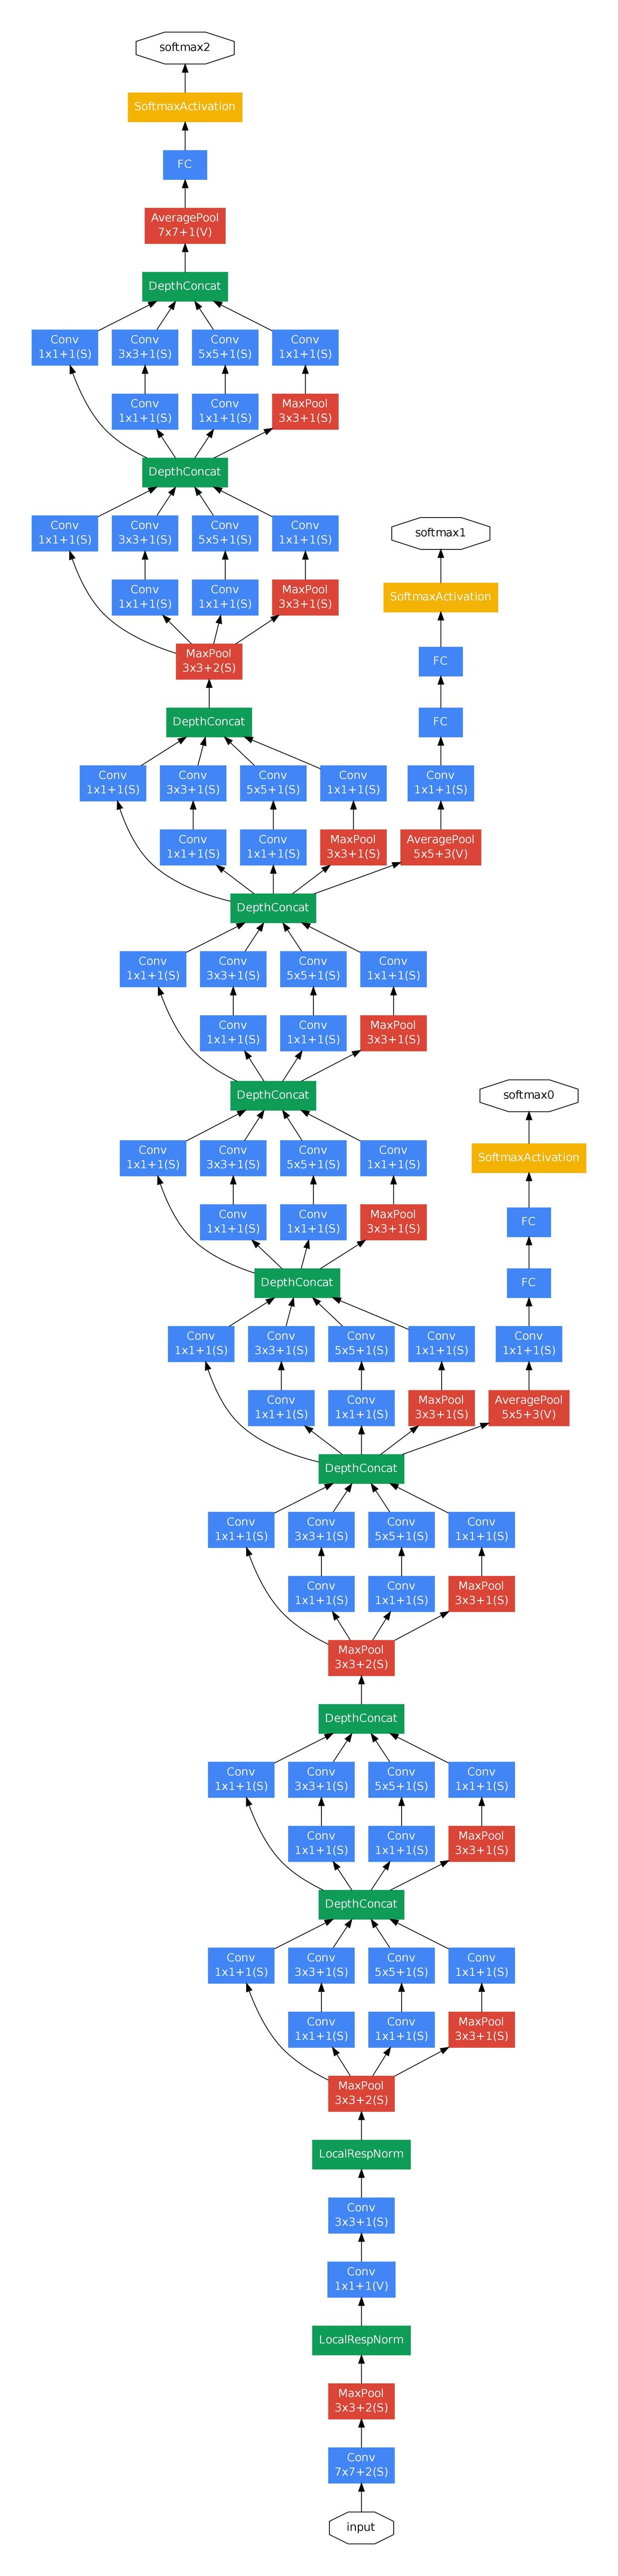
\includegraphics[width=0.4\linewidth]{readings_figures/GoogLeNet_net.jpeg}
	\caption{GoogLeNet网络结构}
	\label{fig:GoogLeNet_net}
\end{figure}

\begin{enumerate}
	\item 输入图像$224\times224\times3$,预处理是图像每个像素减去均值(零均值化);
	\item 卷积层1,$7\times7$,stride:2,padding:3,64通道,输出$112\times112\times64$,卷积后ReLU操作;
	\item 池化层,最大池化,$3\times3$,stride:2,输出$56\times56\times64$,后接ReLU操作;
	\item 卷积层2,$3\times3$,stride:1,padding:1,192通道,输出$56\times56\times192$,卷积后ReLU操作;
	\item 池化层,最大池化,$3\times3$,stride:2,输出$28\times28\times192$,后接ReLU操作;
	\item
	      \begin{itemize}
		      \item inception(3a)
		      \item $1\times1$卷积核,64通道,输出$28\times28\times64$,后接ReLU;
		      \item $1\times1$卷积核,96通道,得到$28\times28\times96$,后接ReLU,$3\times3$卷积核,padding为1,通道128,输出到$28\times28\times128$;
		      \item $1\times1$卷积核,16通道,得到$28\times28\times16$,后接ReLU,$5\times5$卷积核,padding为2,通道32,输出到$28\times28\times32$;
		      \item 最大池化,$3\times3$卷积核,padding为1,通道192,得到$28\times28\times192$,$1\times1$卷积核,32通道,得到$28\times28\times32$;
		      \item 四个部分连接,$64+128+32+32=256$,得到$28\times28\times256$;
	      \end{itemize}
	\item
	      \begin{itemize}
		      \item inception(3b)
		      \item $1\times1$卷积核,128通道,输出$28\times28\times128$,后接ReLU;
		      \item $1\times1$卷积核,128通道,得到$28\times28\times128$,后接ReLU,$3\times3$卷积核,padding为1,通道192,输出到$28\times28\times192$;
		      \item $1\times1$卷积核,32通道,得到$28\times28\times32$,后接ReLU,$5\times5$卷积核,padding为2,通道96,输出到$28\times28\times96$;
		      \item 最大池化,$3\times3$卷积核,padding为1,通道256,得到$28\times28\times256$,$1\times1$卷积核,64通道,得到$28\times28\times64$;
		      \item 四个部分连接,$128+192+96+64=480$,得到$28\times28\times480$;
	      \end{itemize}
	\item 池化层,最大池化,$3\times3$,stride:2,padding:1,输出$14\times14\times480$,后接ReLU操作;
	\item
	      \begin{itemize}
		      \item inception(4a)
		      \item $1\times1$卷积核,192通道,输出$14\times14\times192$,后接ReLU;
		      \item $1\times1$卷积核,96通道,得到$14\times14\times96$,后接ReLU,$3\times3$卷积核,padding为1,通道208,输出到$14\times14\times208$;
		      \item $1\times1$卷积核,16通道,得到$14\times14\times16$,后接ReLU,$5\times5$卷积核,padding为2,通道48,输出到$14\times14\times48$;
		      \item 最大池化,$3\times3$卷积核,padding为1,通道480,得到$14\times14\times480$,$1\times1$卷积核,64通道,得到$14\times14\times64$;
		      \item 四个部分连接,$192+208+48+64=512$,得到$14\times14\times512$;
	      \end{itemize}
	\item
	      \begin{itemize}
		      \item inception(4b)
		      \item $1\times1$卷积核,160通道,输出$14\times14\times160$,后接ReLU;
		      \item $1\times1$卷积核,112通道,得到$14\times14\times112$,后接ReLU,$3\times3$卷积核,padding为1,通道224,输出到$14\times14\times224$;
		      \item $1\times1$卷积核,24通道,得到$14\times14\times24$,后接ReLU,$5\times5$卷积核,padding为2,通道64,输出到$14\times14\times64$;
		      \item 最大池化,$3\times3$卷积核,padding为1,通道512,得到$14\times14\times512$,$1\times1$卷积核,64通道,得到$14\times14\times64$;
		      \item 四个部分连接,$160+224+64+64=512$,得到$14\times14\times512$;
	      \end{itemize}
	\item
	      \begin{itemize}
		      \item inception(4c)
		      \item $1\times1$卷积核,128通道,输出$14\times14\times128$,后接ReLU;
		      \item $1\times1$卷积核,128通道,得到$14\times14\times128$,后接ReLU,$3\times3$卷积核,padding为1,通道256,输出到$14\times14\times256$;
		      \item $1\times1$卷积核,24通道,得到$14\times14\times24$,后接ReLU,$5\times5$卷积核,padding为2,通道64,输出到$14\times14\times64$;
		      \item 最大池化,$3\times3$卷积核,padding为1,通道512,得到$14\times14\times512$,$1\times1$卷积核,64通道,得到$14\times14\times64$;
		      \item 四个部分连接,$128+256+64+64=512$,得到$14\times14\times512$;
	      \end{itemize}
	\item
	      \begin{itemize}
		      \item inception(4d)
		      \item $1\times1$卷积核,112通道,输出$14\times14\times112$,后接ReLU;
		      \item $1\times1$卷积核,144通道,得到$14\times14\times144$,后接ReLU,$3\times3$卷积核,padding为1,通道288,输出到$14\times14\times288$;
		      \item $1\times1$卷积核,32通道,得到$14\times14\times32$,后接ReLU,$5\times5$卷积核,padding为2,通道64,输出到$14\times14\times64$;
		      \item 最大池化,$3\times3$卷积核,padding为1,通道512,得到$14\times14\times512$,$1\times1$卷积核,64通道,得到$14\times14\times64$;
		      \item 四个部分连接,$112+288+64+64=528$,得到$14\times14\times528$;
	      \end{itemize}
	\item
	      \begin{itemize}
		      \item inception(4e)
		      \item $1\times1$卷积核,256通道,输出$14\times14\times256$,后接ReLU;
		      \item $1\times1$卷积核,160通道,得到$14\times14\times160$,后接ReLU,$3\times3$卷积核,padding为1,通道320,输出到$14\times14\times320$;
		      \item $1\times1$卷积核,32通道,得到$14\times14\times32$,后接ReLU,$5\times5$卷积核,padding为2,通道128,输出到$14\times14\times128$;
		      \item 最大池化,$3\times3$卷积核,padding为1,通道528,得到$14\times14\times528$,$1\times1$卷积核,128通道,得到$14\times14\times128$;
		      \item 四个部分连接,$256+320+128+128=832$,得到$14\times14\times832$;
	      \end{itemize}
	\item 池化层,最大池化,$3\times3$,stride:2,padding:1,输出$7\times7\times832$,后接ReLU操作;
	\item
	      \begin{itemize}
		      \item inception(5a)
		      \item $1\times1$卷积核,256通道,输出$7\times7\times256$,后接ReLU;
		      \item $1\times1$卷积核,160通道,得到$7\times7\times160$,后接ReLU,$3\times3$卷积核,padding为1,通道320,输出到$7\times7\times320$;
		      \item $1\times1$卷积核,32通道,得到$7\times7\times32$,后接ReLU,$5\times5$卷积核,padding为2,通道128,输出到$7\times7\times128$;
		      \item 最大池化,$3\times3$卷积核,padding为1,通道832,得到$7\times7\times832$,$1\times1$卷积核,128通道,得到$7\times7\times128$;
		      \item 四个部分连接,$256+320+128+128=832$,得到$7\times7\times832$;
	      \end{itemize}
	\item
	      \begin{itemize}
		      \item inception(5b)
		      \item $1\times1$卷积核,384通道,输出$7\times7\times384$,后接ReLU;
		      \item $1\times1$卷积核,192通道,得到$7\times7\times192$,后接ReLU,$3\times3$卷积核,padding为1,通道384,输出到$7\times7\times384$;
		      \item $1\times1$卷积核,48通道,得到$7\times7\times48$,后接ReLU,$5\times5$卷积核,padding为2,通道128,输出到$7\times7\times128$;
		      \item 最大池化,$3\times3$卷积核,padding为1,通道832,得到$7\times7\times832$,$1\times1$卷积核,128通道,得到$7\times7\times128$;
		      \item 四个部分连接,$384+384+128+128=1024$,得到$7\times7\times1024$;
	      \end{itemize}
	\item 池化层,平均池化,$7\times7$,stride:1,输出$1\times1\times1024$,后接ReLU操作;
	\item dropout(40\%),输出$1\times1\times1024$;
	\item linear,输入$1\times1024$,输出$1\times1000$;
	\item softmax,输出$1\times1000$;
\end{enumerate}

网络的相关参数设置如下~\ref{fig:GoogLeNet_params}所示,其中$\#3\times3\ reduce$和$\#5\times5\ reduce$表示在卷积之前,进行降维使用的$1\times1$的滤波器数量。

\begin{figure}[htbp]
	\centering
	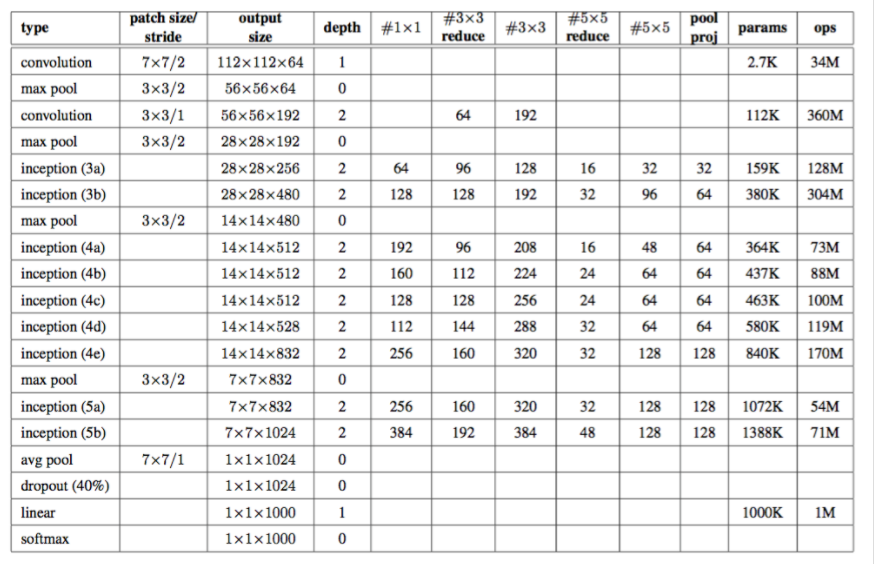
\includegraphics[width=\linewidth]{readings_figures/GoogLeNet_params.png}
	\caption{GoogLeNet网络参数设置}
	\label{fig:GoogLeNet_params}
\end{figure}

\section{inception v2 v3}

在提出了Inception v1结构之后,Google团队在\cite{ioffe2015batch}中提到训练深度神经网络的复杂性在于,由于前面的层的参数在训练过程中会发生变化,这就导致了后面的层是输入的分布在训练过程中也会发生改变;并且由于网络层数的加深,网络参数细微的变化会被逐渐放大;较低的学习率和仔细地参数初始化也导致了模型的训练速度变慢,同时使得具有饱和非线性的模型训练起来十分困难,这种现象被称为内部协变量转移。为此,该文章中又提出了批标准化BN来解决该问题。将标准化做成模型架构的一部分,并为每个批量小数据做标准化,可以在不用太注意学习率初始化的同时提高学习率,同时作为一个正则化项,使得网络可以去除Dropout。应用于其他的图像分类模型之后,在达到相同精度的情况下,能够缩小14倍的训练步骤,并以显著的差距击败了原始模型。

2016年,Szegedy等人\cite{szegedy2016rethinking}针对计算效率限制了卷积网络具体场景上的应用的问题,探索了增大网络的方法,通过适当的卷积和正则化来尽可能提高计算效率。

Inception架构的复杂性使得难以对网络进行更改,单纯地方法架构会导致计算效率的降低,为此需要使用一些具有卷积网络、具有各种架构选择和基于大规模实验的设计原则。在网络的前面尽量避免表征瓶颈;更高维度的表示在网络中更容易局部处理;空间聚合可以在较低维度嵌入上完成,而不会在表示能力上造成许多损失;最后是需要平衡每个阶段的滤波器数量和网络深度以使网络达到较好性能。

在文章中,作者提出了一些新的想法:

\begin{figure}[htbp]
	\centering
	\subfloat[Inception v2 3x3 convolutions]{
		\centering
		\begin{minipage}{0.40\linewidth}
			\centering
			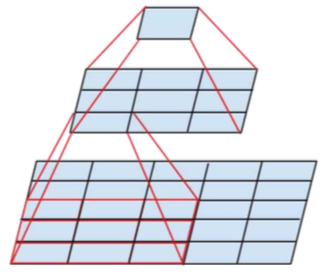
\includegraphics[width = \linewidth]{readings_figures/Inception_v2_3x3.png}
			\label{fig:Inception_v2_3x3_convolutions}
		\end{minipage}
	}
	\centering
	\subfloat[Inception v2 3x1 convolutions]{
		\centering
		\begin{minipage}{0.40\linewidth}
			\centering
			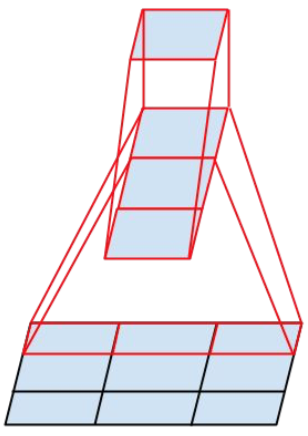
\includegraphics[width = \linewidth]{readings_figures/Inception_v2_3x1.png}
			\label{fig:Inception_v2_3x1_convolutions}
		\end{minipage}
	}
	\centering
	\caption{Inception v2 卷积核替代}
	\label{fig:Inception_v2_convolutions}
\end{figure}

卷积分解,如图~\ref{fig:Inception_v2_3x3_convolutions}一个$5\times5$的卷积可由两个$3\times3$的卷积核进行替代,在保证了有$5\times5$的卷积核的感受野的同时,在一定程度上减少了参数量。因此,大于$3\times3$的滤波器并不总是有用的,因为总可以用$3\times3$的卷积核来简化。更进一步想,是否通过分解成更小的卷积核例如$2\times2$的卷积。但是,论文中提到通过非对称卷积即$n\times1$甚至可以做出比$2\times2$卷积更好的效果,$3\times1$的卷积后面接$1\times3$的卷积~\ref{fig:Inception_v2_3x1_convolutions}相当于以$3\times3$的卷积的感受野滑动两层网络。因此,改进的两种新的Inception架构如图~\ref{fig:Inception_module_convolutions},进一步可改进为~\ref{fig:Inception_module_with_expand}。

\begin{figure}[htbp]
	\centering
	\subfloat[Inception v1 module 5x5 convolutions]{
		\centering
		\begin{minipage}{0.30\linewidth}
			\centering
			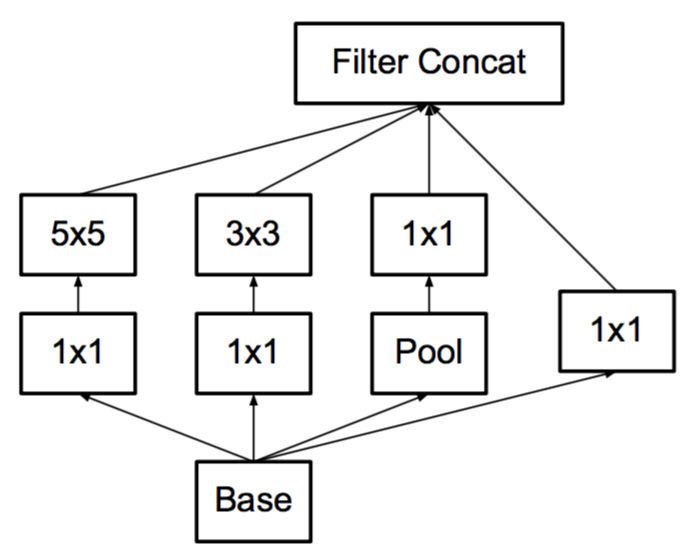
\includegraphics[width = \linewidth]{readings_figures/Inception_v1_module_5x5.png}
			\label{fig:Inception_v1_module_5x5_convolutions}
		\end{minipage}
	}
	\centering
	\subfloat[Inception v2 module 3x3 convolutions]{
		\centering
		\begin{minipage}{0.30\linewidth}
			\centering
			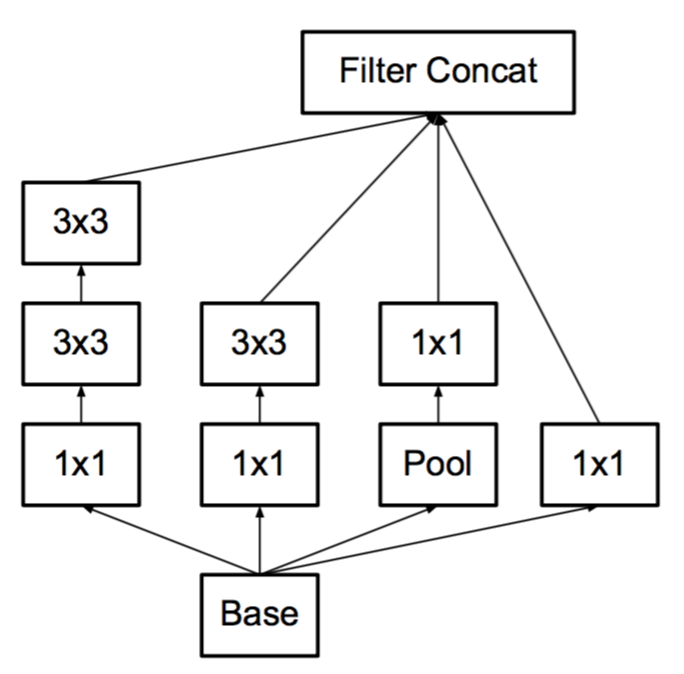
\includegraphics[width = \linewidth]{readings_figures/Inception_v2_module_3x3.png}
			\label{fig:Inception_v2_module_3x3_convolutions}
		\end{minipage}
	}
	\centering
	\subfloat[Inception v3 module 3x1 convolutions]{
		\centering
		\begin{minipage}{0.30\linewidth}
			\centering
			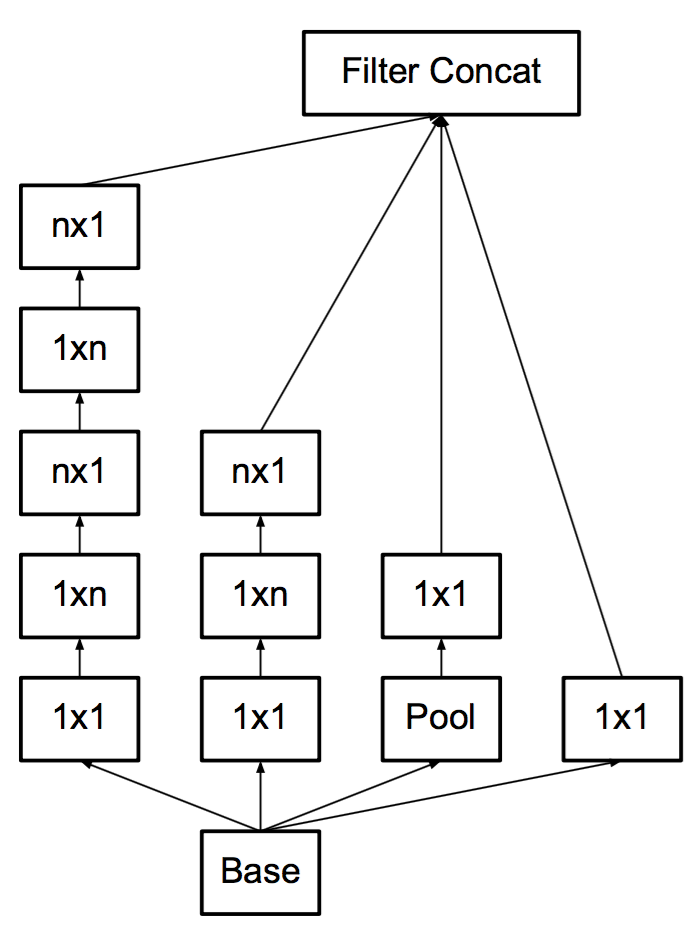
\includegraphics[width = \linewidth]{readings_figures/Inception_v3_module_3x1.png}
			\label{fig:Inception_v3_module_3x1_convolutions}
		\end{minipage}
	}
	\centering
	\caption{Inception 改进架构}
	\label{fig:Inception_module_convolutions}
\end{figure}

\begin{figure}[htbp]
	\centering
	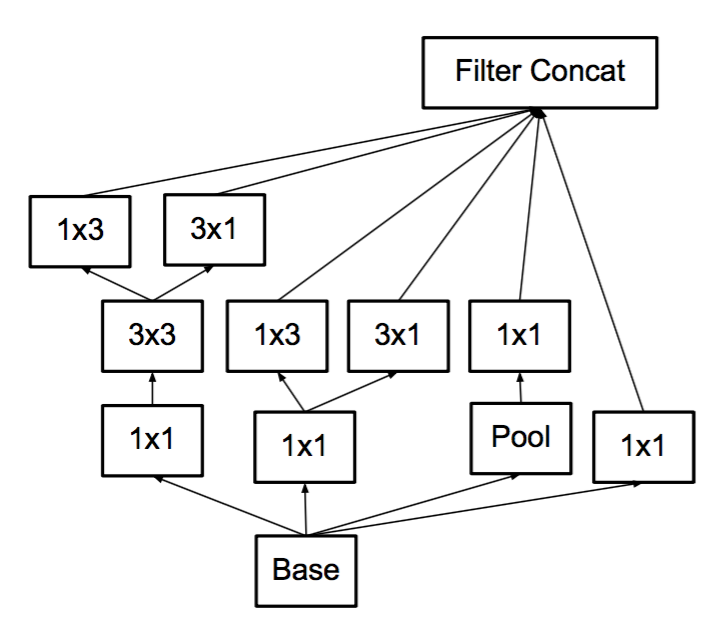
\includegraphics[width=\linewidth]{readings_figures/Inception_module_with_expand.png}
	\caption{Inception module改进}
	\label{fig:Inception_module_with_expand}
\end{figure}

有效减小网格尺寸,作者对Inception进行了改进,假设开始有一个带有k个滤波器的d×d网格,如果我们想要达到一个带有2k个滤波器的$\frac{d}{2}\times\frac{d}{2}$网格,现有以下两种方案~\ref{fig:Origin_grid_size},左边是转换为带有卷积的池化,将计算成本降为原来的$\frac{1}{4}$,但是这样将会导致网络产生瓶颈;右边则是先采用$1\times1$卷积进行升维,再进行池化缩小尺寸,但这样无疑会导致计算量巨大。为此,产生了另一种变体~\ref{fig:Inception_grid_size},使用两个平行的步长为2的块,改进后的Inception模块具有缩小特征图尺寸的功能,左图是具体的操作方式,右图从特征图尺寸角度说明。

\begin{figure}[htbp]
	\centering
	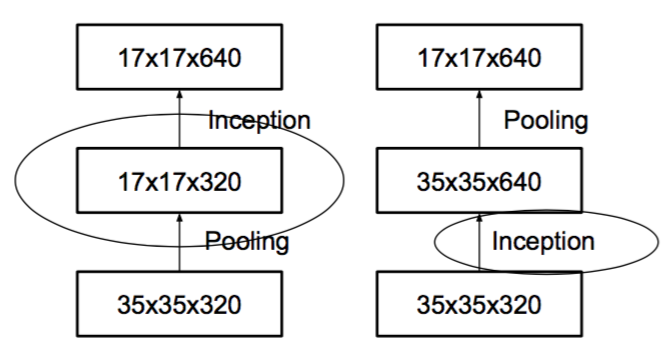
\includegraphics[width=\linewidth]{readings_figures/Origin_grid_size.png}
	\caption{原始减小网格尺寸方法}
	\label{fig:Origin_grid_size}
\end{figure}

\begin{figure}[htbp]
	\centering
	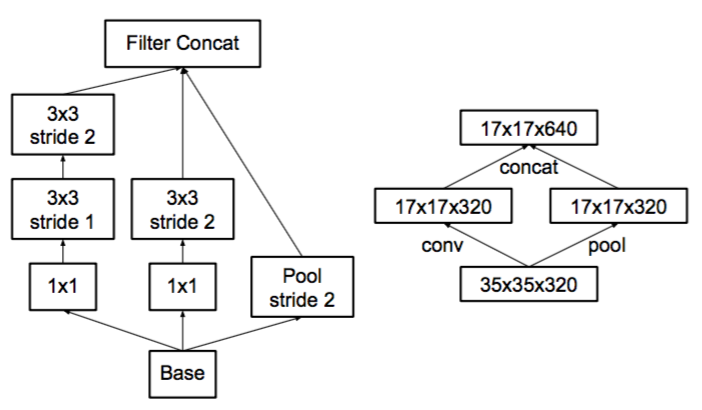
\includegraphics[width=\linewidth]{readings_figures/Inception_grid_size.png}
	\caption{Inception减小网格尺寸方法}
	\label{fig:Inception_grid_size}
\end{figure}

Inception v2的结构如~\ref{fig:Inception_v2_module},图中的figure5对应~\ref{fig:Inception_v2_module_3x3_convolutions},figure6对应~\ref{fig:Inception_v3_module_3x1_convolutions},figure7对应~\ref{fig:Inception_module_with_expand}

\begin{figure}[htbp]
	\centering
	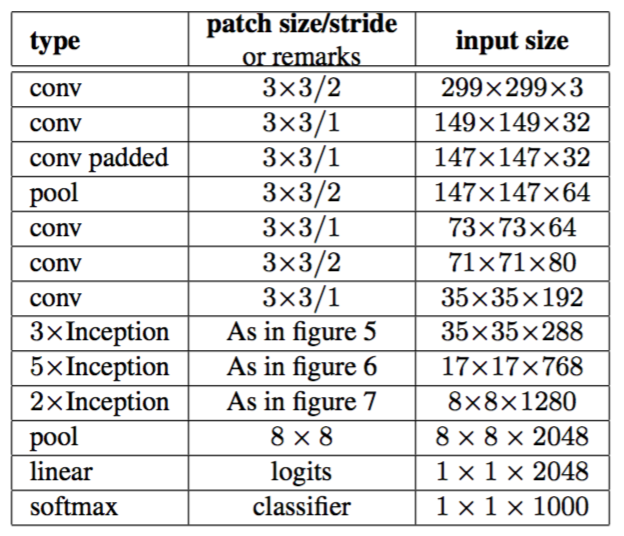
\includegraphics[width=0.5\linewidth]{readings_figures/Inception_v2_module.png}
	\caption{Inception v2结构}
	\label{fig:Inception_v2_module}
\end{figure}

作者等人在k=1000类的ImageNet比赛中进行了模型的测试,结果如~\ref{fig:Inception_v2_v3_result},在Inception-v2行之后,变化是累积的,每一行都包含除了前面的变化之外的新变化。

\begin{figure}[htbp]
	\centering
	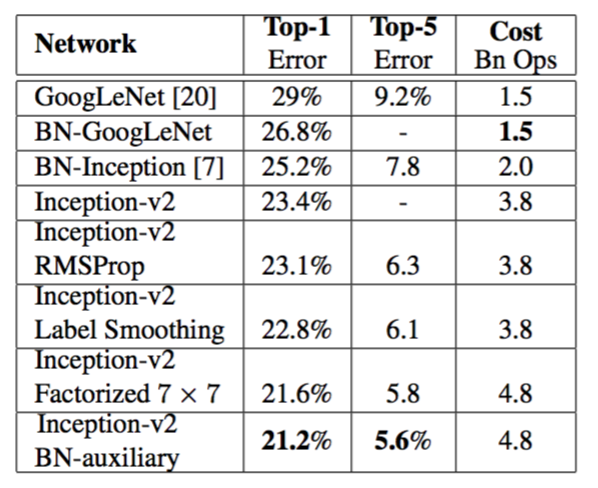
\includegraphics[width=0.5\linewidth]{readings_figures/Inception_v2_v3_result.png}
	\caption{Inception 测试结果}
	\label{fig:Inception_v2_v3_result}
\end{figure}

Inception v3的结构与Inception v2的结构类似,只是将~\ref{fig:Inception_v2_v3_result}中Inception-v2的所有变化都包含了。

\section{inception v4}

在ResNet提出之后,Szegedy等人\cite{szegedy2017inception}考虑到残差模块对于较深的网络具有较大的意义,而Inception网络普遍比较深,于是提出了是否可以将残差网络与Inception module结合起来,结果证实了可以显著提高网络的性能。

Inception v4并没有用到残差网络的思想,而是在Inception v2和v3的基础上进行了简化得到的,网络结构如~\ref{fig:Inception_v4_model}。

\begin{figure}[htbp]
	\centering
	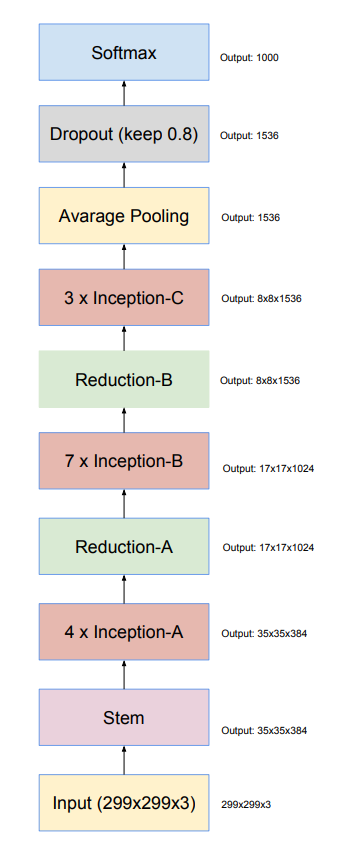
\includegraphics[width=0.6\linewidth]{readings_figures/Inception_v4_model.png}
	\caption{Inception v4}
	\label{fig:Inception_v4_model}
\end{figure}

其中包含有:
stem结构~\ref{fig:Inception_v4_stem}:

\begin{figure}[htbp]
	\centering
	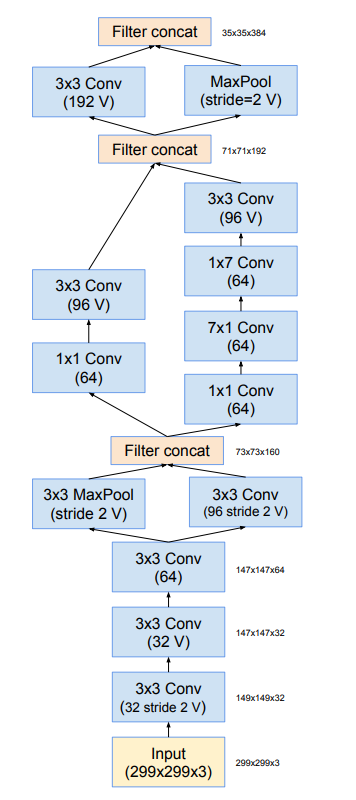
\includegraphics[width=0.7\linewidth]{readings_figures/Inception_v4_stem.png}
	\caption{Inception v4 stem}
	\label{fig:Inception_v4_stem}
\end{figure}

3个Inception基本模块~\ref{fig:Inception_v4_inception_module}:

\begin{figure}[htbp]
	\centering
	\subfloat[Inception v4 module 35x35 grid]{
		\centering
		\begin{minipage}{0.30\linewidth}
			\centering
			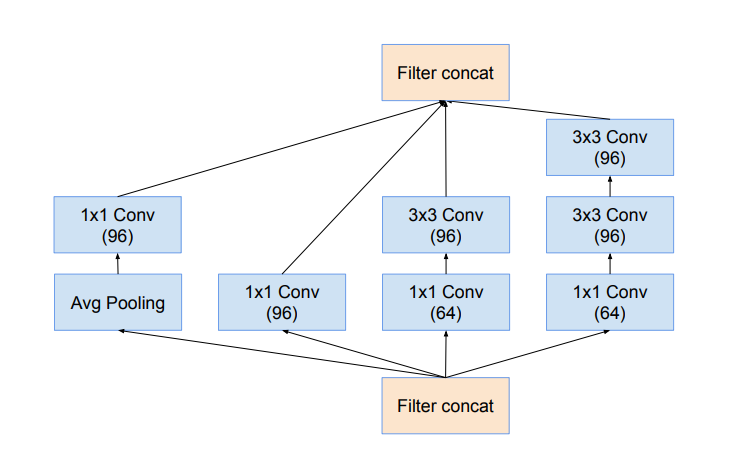
\includegraphics[width = \linewidth]{readings_figures/Inception_v4_35grid.png}
			\label{fig:Inception_v4_35grid}
		\end{minipage}
	}
	\centering
	\subfloat[Inception v4 module 17x17 grid]{
		\centering
		\begin{minipage}{0.30\linewidth}
			\centering
			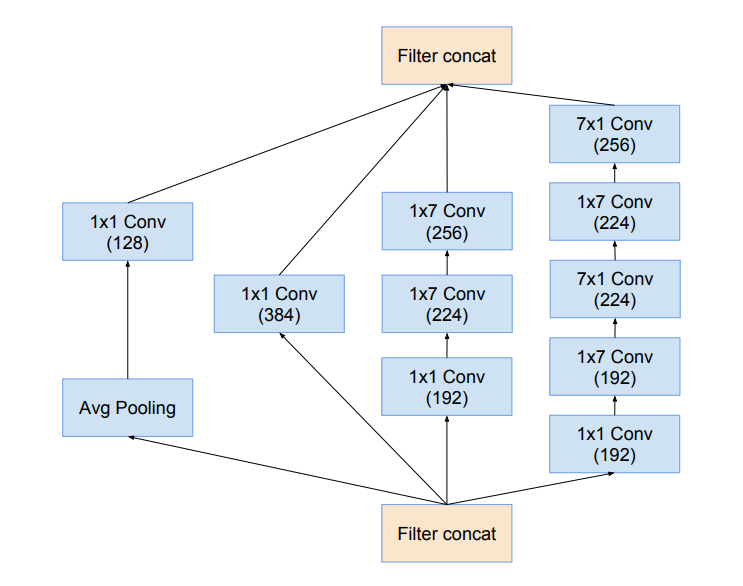
\includegraphics[width = \linewidth]{readings_figures/Inception_v4_17grid.png}
			\label{fig:Inception_v4_17grid}
		\end{minipage}
	}
	\centering
	\subfloat[Inception v4 module 8x8 grid]{
		\centering
		\begin{minipage}{0.30\linewidth}
			\centering
			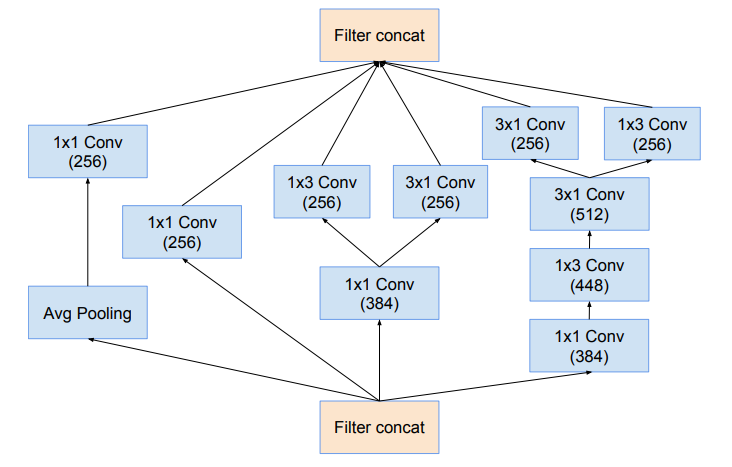
\includegraphics[width = \linewidth]{readings_figures/Inception_v4_8grid.png}
			\label{fig:Inception_v4_8grid}
		\end{minipage}
	}
	\centering
	\caption{Inception v4 基本模块}
	\label{fig:Inception_v4_inception_module}
\end{figure}

2个过渡模块~\ref{fig:Inception_v4_inception_grid_change_module}:

\begin{figure}[htbp]
	\centering
	\subfloat[Inception v4 module 35to17]{
		\centering
		\begin{minipage}{0.30\linewidth}
			\centering
			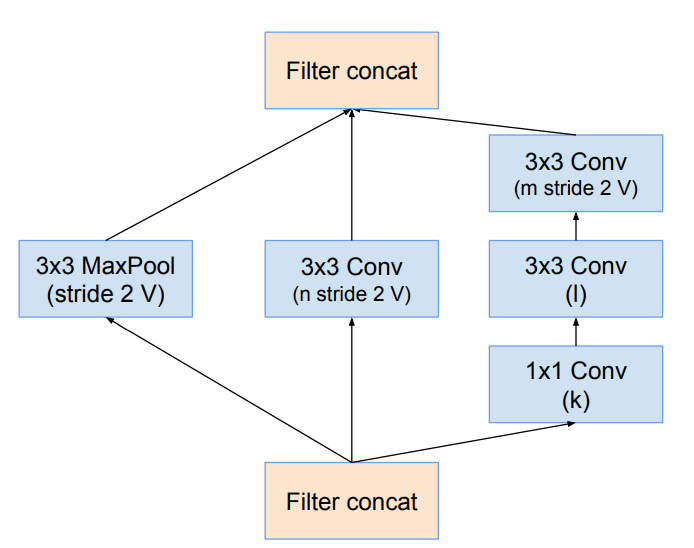
\includegraphics[width = \linewidth]{readings_figures/Inception_v4_35to17grid.png}
			\label{fig:Inception_v4_35to17}
		\end{minipage}
	}
	\centering
	\subfloat[Inception v4 module 17to8]{
		\centering
		\begin{minipage}{0.30\linewidth}
			\centering
			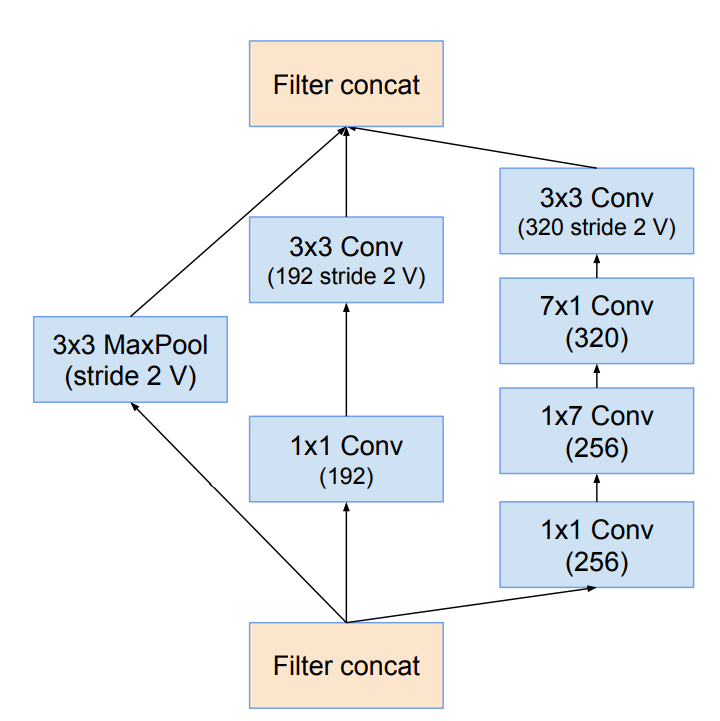
\includegraphics[width = \linewidth]{readings_figures/Inception_v4_17to8grid.png}
			\label{fig:Inception_v4_17to8}
		\end{minipage}
	}
	\centering
	\caption{Inception v4 过渡模块}
	\label{fig:Inception_v4_inception_grid_change_module}
\end{figure}

在Inception v4的同篇文章中,作者等人将残差网络的思想与Inception结构结合起来,提出了Inception-ResNet-v1和Inception-ResNet-v2的网络,两者的网络结构相同~\ref{fig:Inception_ResNet_model},不同是中间使用的组件不同。

\begin{figure}[htbp]
	\centering
	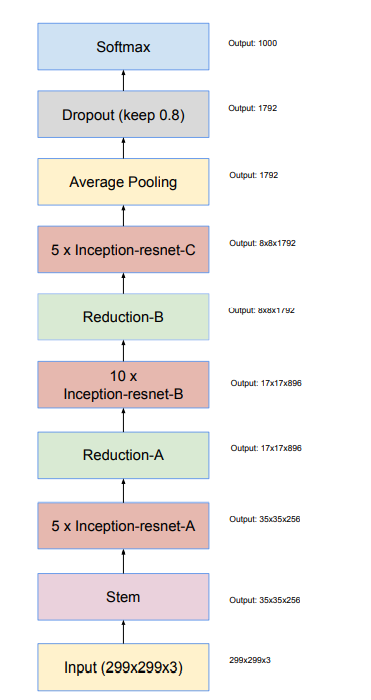
\includegraphics[width=0.6\linewidth]{readings_figures/Inception_ResNet_model.png}
	\caption{Inception ResNet 网络结构}
	\label{fig:Inception_ResNet_model}
\end{figure}

Inception-ResNet-v1使用~\ref{fig:Inception_ResNet_v1_stem}的stem结构,~\ref{fig:Inception_ResNet_v1_35grid}、~\ref{fig:Inception_ResNet_v1_17grid}和~\ref{fig:Inception_ResNet_v1_8grid}的基本结构,~\ref{fig:Inception_v4_35to17}和~\ref{fig:Inception_ResNet_v1_17to8}的过渡模块;

\begin{figure}[htbp]
	\centering
	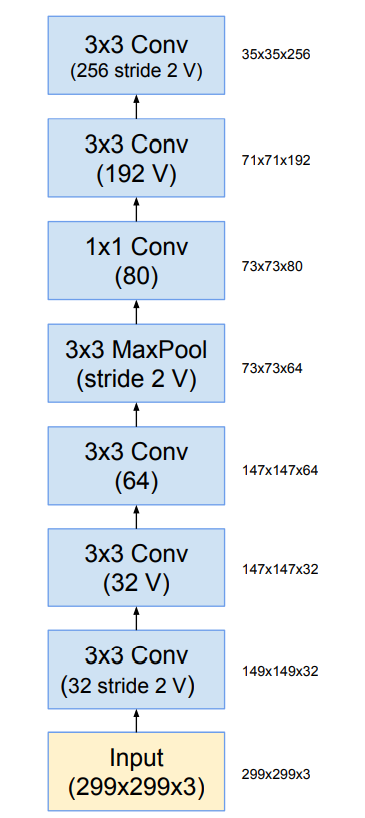
\includegraphics[width=0.7\linewidth]{readings_figures/Inception_ResNet_v1_stem.png}
	\caption{Inception ResNet v1 stem结构}
	\label{fig:Inception_ResNet_v1_stem}
\end{figure}

\begin{figure}[htbp]
	\centering
	\subfloat[Inception-ResNet-v1 module 35x35 grid]{
		\centering
		\begin{minipage}{0.30\linewidth}
			\centering
			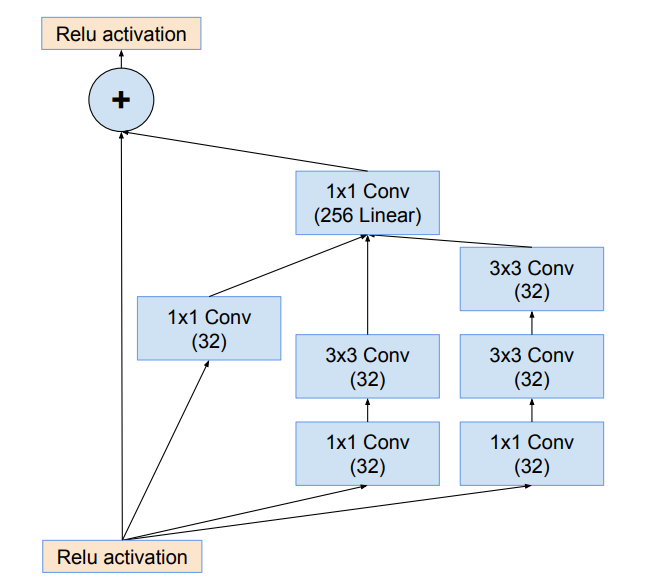
\includegraphics[width = \linewidth]{readings_figures/Inception_ResNet_v1_35grid.png}
			\label{fig:Inception_ResNet_v1_35grid}
		\end{minipage}
	}
	\centering
	\subfloat[Inception-ResNet-v1 module 17x17 grid]{
		\centering
		\begin{minipage}{0.30\linewidth}
			\centering
			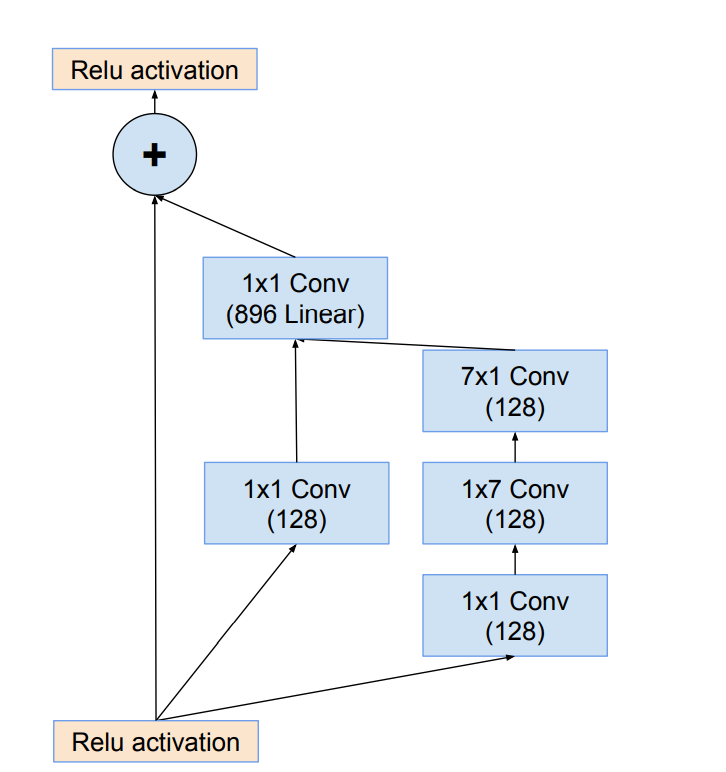
\includegraphics[width = \linewidth]{readings_figures/Inception_ResNet_v1_17grid.png}
			\label{fig:Inception_ResNet_v1_17grid}
		\end{minipage}
	}
	\\
	\centering
	\subfloat[Inception-ResNet-v1 module 8x8 grid]{
		\centering
		\begin{minipage}{0.30\linewidth}
			\centering
			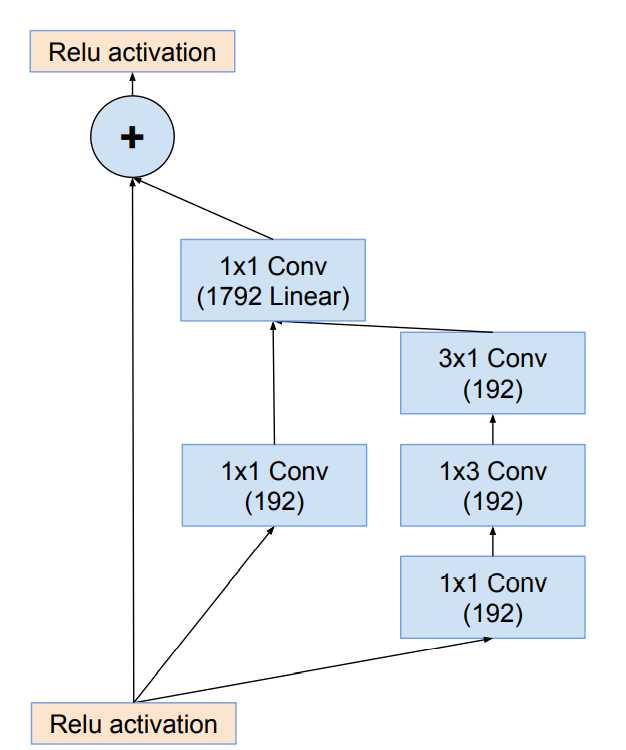
\includegraphics[width = \linewidth]{readings_figures/Inception_ResNet_v1_8grid.png}
			\label{fig:Inception_ResNet_v1_8grid}
		\end{minipage}
	}
	\centering
	\subfloat[Inception-ResNet-v1 module 17to8]{
		\centering
		\begin{minipage}{0.30\linewidth}
			\centering
			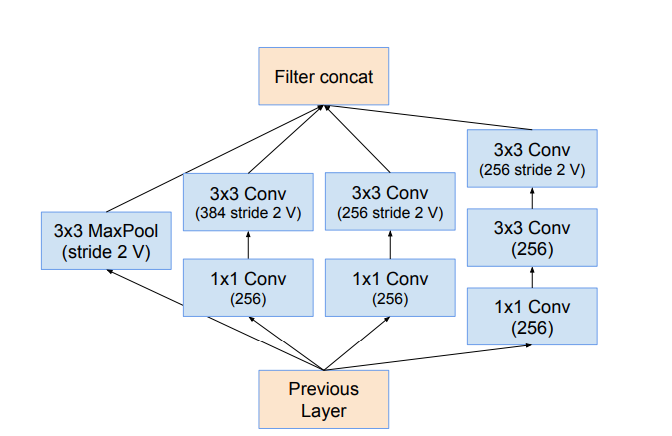
\includegraphics[width = \linewidth]{readings_figures/Inception_ResNet_v1_17to8grid.png}
			\label{fig:Inception_ResNet_v1_17to8}
		\end{minipage}
	}
	\centering
	\caption{Inception-ResNet-v1 模块}
	\label{fig:Inception_ResNet_v1_module}
\end{figure}

Inception-ResNet-v2使用~\ref{fig:Inception_v4_stem}的stem结构,~\ref{fig:Inception_ResNet_v2_35grid}、~\ref{fig:Inception_ResNet_v2_17grid}和~\ref{fig:Inception_ResNet_v2_8grid}的基本结构,~\ref{fig:Inception_v4_35to17}和~\ref{fig:Inception_ResNet_v2_17to8}的过渡模块。

\begin{figure}[htbp]
	\centering
	\subfloat[Inception-ResNet-v2 module 35x35 grid]{
		\centering
		\begin{minipage}{0.30\linewidth}
			\centering
			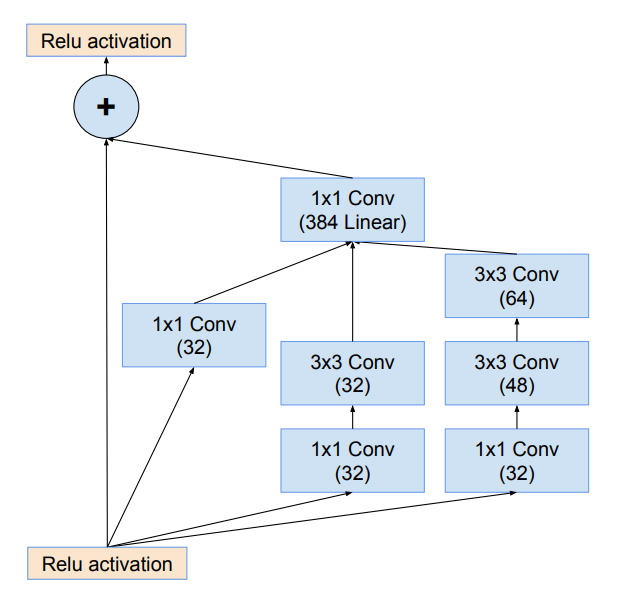
\includegraphics[width = \linewidth]{readings_figures/Inception_ResNet_v2_35grid.png}
			\label{fig:Inception_ResNet_v2_35grid}
		\end{minipage}
	}
	\centering
	\subfloat[Inception-ResNet-v2 module 17x17 grid]{
		\centering
		\begin{minipage}{0.30\linewidth}
			\centering
			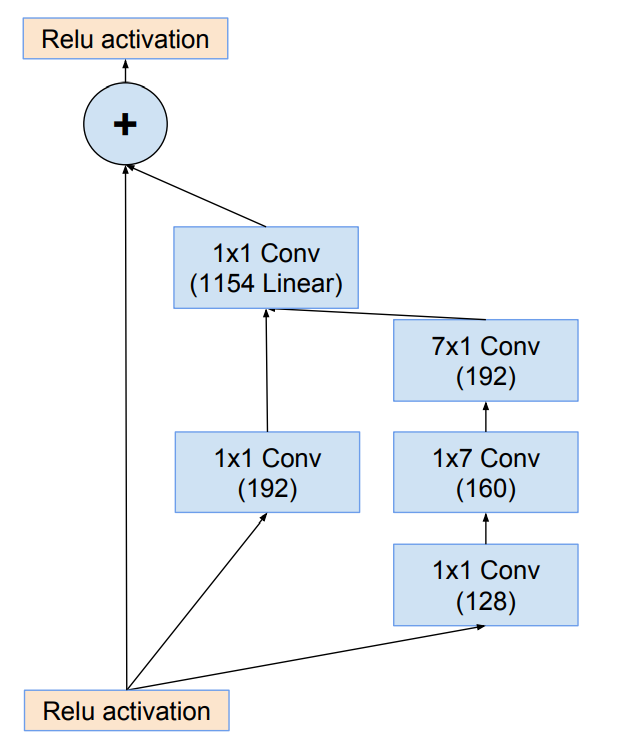
\includegraphics[width = \linewidth]{readings_figures/Inception_ResNet_v2_17grid.png}
			\label{fig:Inception_ResNet_v2_17grid}
		\end{minipage}
	}
	\\
	\centering
	\subfloat[Inception-ResNet-v2 module 8x8 grid]{
		\centering
		\begin{minipage}{0.30\linewidth}
			\centering
			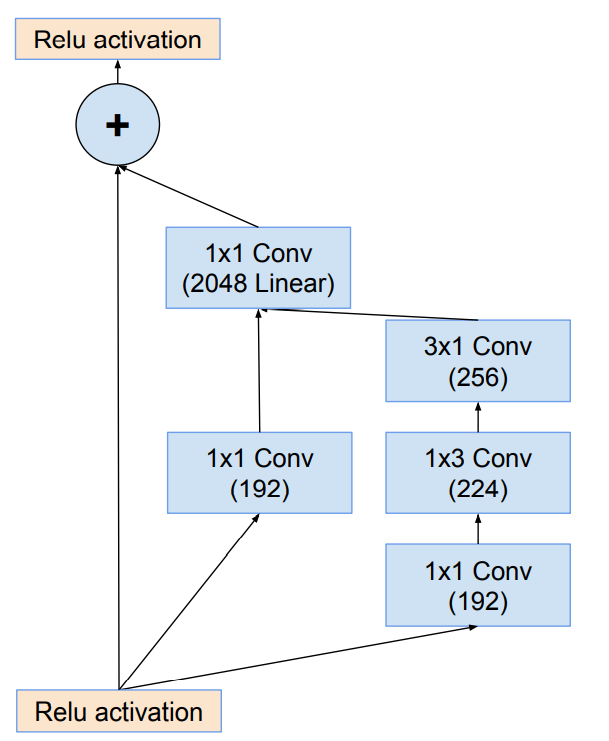
\includegraphics[width = \linewidth]{readings_figures/Inception_ResNet_v2_8grid.png}
			\label{fig:Inception_ResNet_v2_8grid}
		\end{minipage}
	}
	\centering
	\subfloat[Inception-ResNet-v2 module 17to8]{
		\centering
		\begin{minipage}{0.30\linewidth}
			\centering
			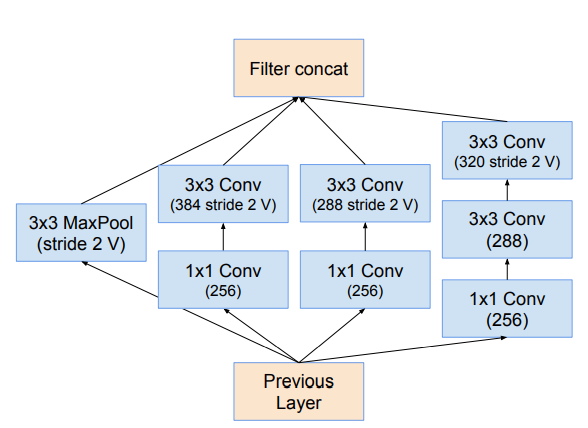
\includegraphics[width = \linewidth]{readings_figures/Inception_ResNet_v2_17to8grid.png}
			\label{fig:Inception_ResNet_v2_17to8}
		\end{minipage}
	}
	\centering
	\caption{Inception-ResNet-v2 模块}
	\label{fig:Inception_ResNet_v2_module}
\end{figure}

\section{ResNet}

He等人\cite{he2016deep}提出的ResNet网络取得了2015年的ILSVRC冠军。

ResNet主要针对神经网络训练过程中的退化问题,文章中提到对浅层神经网络通过堆叠层的数量,随着模型复杂度的提高,可以提高训练的准确率。随着神经网络层数的增加,梯度消失或梯度爆炸是很常见的问题,但是这些都已经通过标准初始化或BN层的引入得到很好地解决。但是,当网络层数很深时,却存在了退化问题:随着网络深度的增加,准确率达到饱和,然后迅速下降,如图~\ref{fig:ResNet_compare_layers}所示。从图中可以看出,当深度达到某一值后,更深的网络具有更高的训练误差和测试误差。为此,ResNet网络从改变模型结构着手,使得模型更易于优化。

\begin{figure}[htbp]
	\centering
	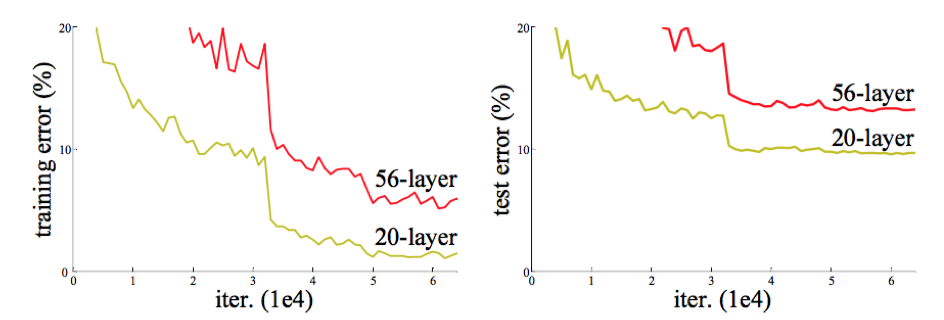
\includegraphics[width=\linewidth]{readings_figures/ResNet_compare_layers.jpeg}
	\caption{训练结果与层数关系}
	\label{fig:ResNet_compare_layers}
\end{figure}

何为残差学习,假设H(x)作为几个堆叠层(不必要是整个网络)要拟合的基础映射,其能够拟合的映射是F(x),x表示这些层中第一层的输入。为此,可以让这些层近似$F(x):=H(x)-x$,而不是期望近似H(x),因此,原始函数变为$F(x)+x$。

\begin{figure}[htbp]
	\centering
	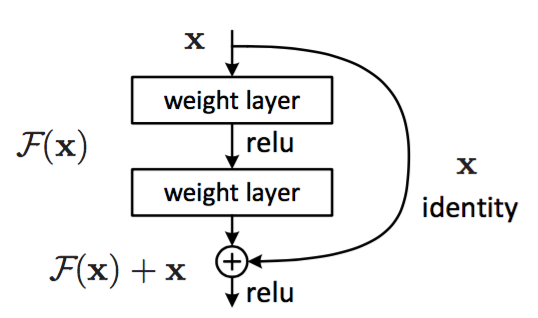
\includegraphics[width=\linewidth]{readings_figures/ResNet_block.jpeg}
	\caption{ResNet block 设计}
	\label{fig:ResNet_block}
\end{figure}

对于这样的堆叠层的设计,被称为block,如图~\ref{fig:ResNet_block},用于计算$F(x)+x$。block中包含有两个路径方向,一是计算残差F(x),另一种是计算x,恒等映射。最后将F(x)与x进行累加,但是需要注意的是两者尺寸必须相同。关于F(x)的计算,则是~\ref{fig:ResNet_block_Fx}中,一种是两个$3\times3$的卷据构成,另一种是通过$1\times1$的卷积先进行降维后升维。x的变化则依据F(x)的不同有所变化,一种是输入x作为输出,另一种是通过$1\times1$的卷积进行维度的改变,以保证x和F(x)的尺寸一致。至于不同block之间的连接,$F(x)+x$进行ReLU之后作为下一个block的输入。

\begin{figure}[htbp]
	\centering
	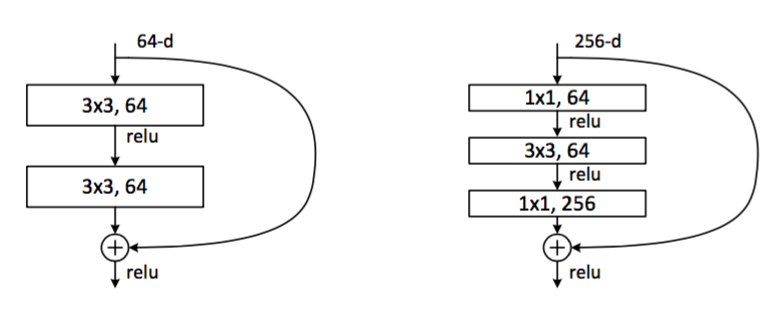
\includegraphics[width=\linewidth]{readings_figures/ResNet_block_Fx.jpeg}
	\caption{ResNet block F(x)计算}
	\label{fig:ResNet_block_Fx}
\end{figure}

\begin{figure}[htbp]
	\centering
	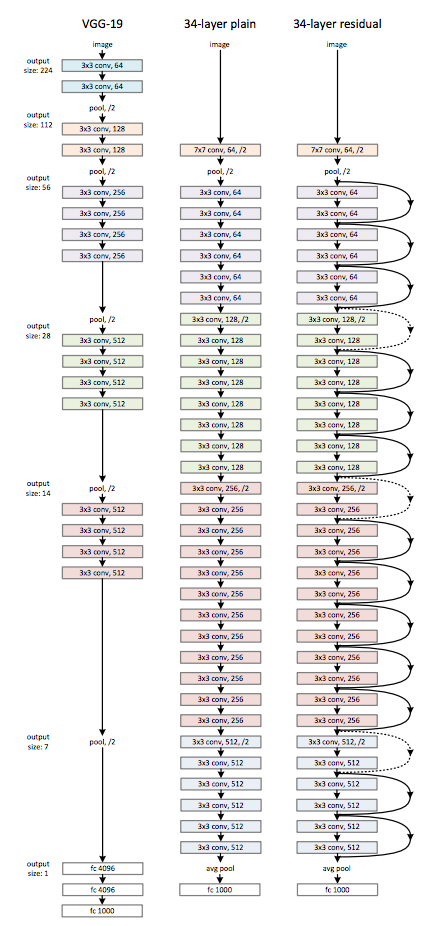
\includegraphics[width=0.8\linewidth]{readings_figures/ResNet_net.jpeg}
	\caption{ResNet网络结构对比图}
	\label{fig:ResNet_net}
\end{figure}


ResNet网络是通过多个block进行堆叠形成的,原文中ResNet34与34层简单网络plain net、VGG网络的对比图如图~\ref{fig:ResNet_net}。网络参数设置如图~\ref{fig:ResNet_params},ResNet的主要特点有:

\begin{enumerate}
	\item ResNet结构是通过堆叠block形成的,与简单网络相比,ResNet中的block多了分支;
	\item ResNet中的下采样是通过$2\times2$的卷积层实现;
	\item ResNet在图中虚线处进行下采样,并升维,即$conv3\_1$,$conv4\_1$,$conv5\_1$处;
	\item 最后采用平均池化,没有全连接层;
	\item 每个卷积层后都接有BN;
\end{enumerate}

\begin{figure}[htbp]
	\centering
	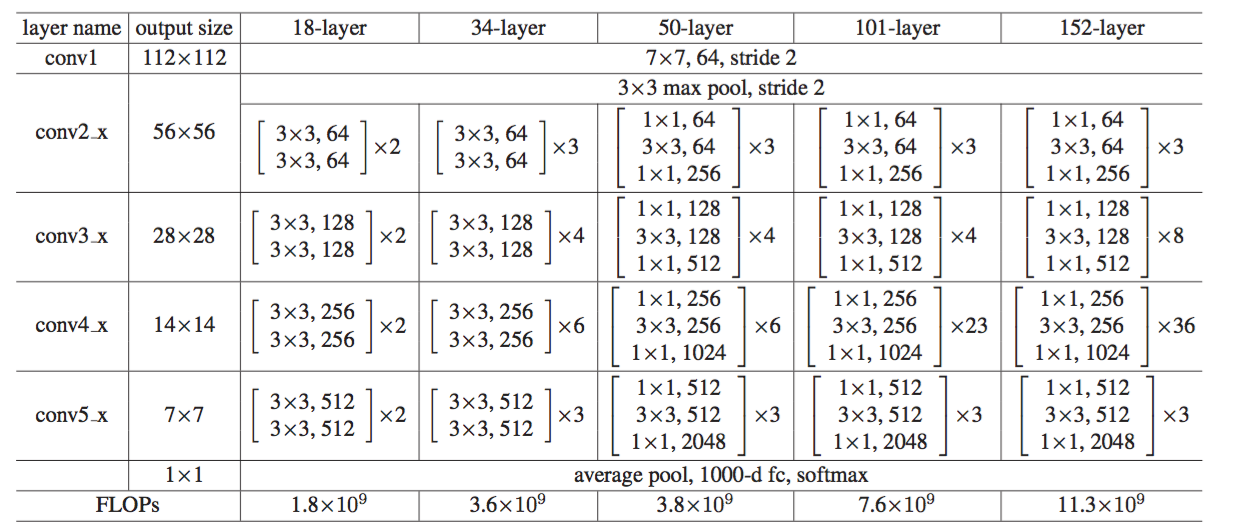
\includegraphics[width=\linewidth]{readings_figures/ResNet_params.jpeg}
	\caption{ResNet网络结构参数图}
	\label{fig:ResNet_params}
\end{figure}

正是由于ResNet使用block进行堆叠,可以通过对block的通道数量以及整个网络的block数量进行修改来调整网络的深度,而不用担心网络的“退化”问题。

\section{DenseNet}

目前已经提出的效果较好的网络结构中,要么是对网络深度进行加深,如Vgg,ResNet通过恒等映射设计了不同深度的网络结构,另一个方向则是对网络进行了加宽,如GoogLeNet中的Inception结构,而Huang等人于2017年提出的DenseNet\cite{huang2017densely}是在尽可能保证网络层与层之间的信息传递,使得特征图能够得到最大程度的利用,获得了CVPR的最佳论文奖。

无论是ResNet还是Highway Networks,或者是FractalNets,尽管在网络结构和训练过程中都一样,但都保持着从前面的层到后面的层的一个短路径。而作者等人为了保证网络中层与层之间拥有最大信息流,则是直接将网络中的所有图层相互连接,即在保证网络前馈的前提下,每个图层获取前面所有图层的输出作为输入,然后将本层的特征图贴到后面共同作为下一层的输入,示意图如~\ref{fig:DenseNet_block}:

\begin{figure}[htbp]
	\centering
	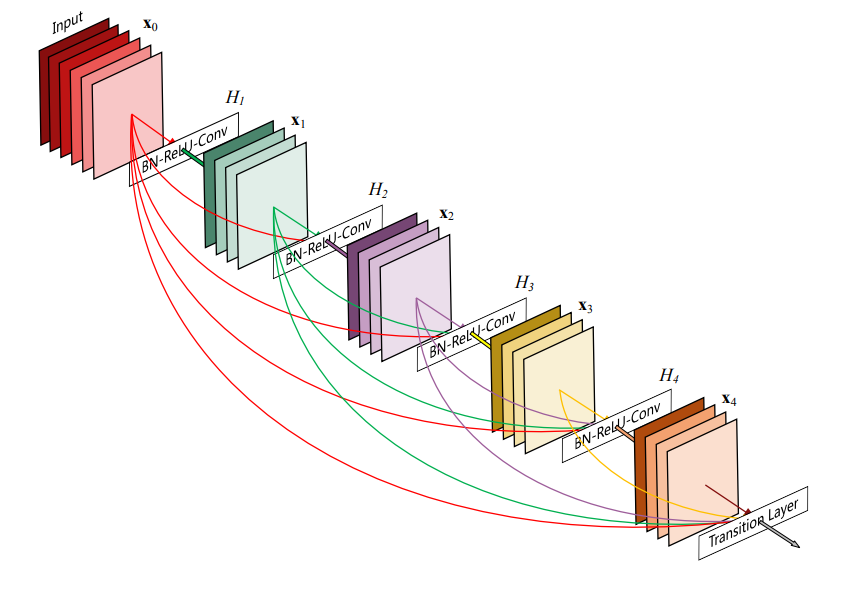
\includegraphics[width=\linewidth]{readings_figures/DenseNet_block.png}
	\caption{DenseNet连接示意图}
	\label{fig:DenseNet_block}
\end{figure}

与传统卷积神经网络不同的是,在卷积神经网络中,有L层,那么会存在L个连接;而在DenseNet中,则会有$\frac{L(L+1)}{2}$个连接。ResNet中,在将特征传给下一层之间会进行相加操作;而在DenseNet中,则是将这些特征图进行拼接,即第l层有l个输入,前面l层的特征图,本层的特征图则传递给之后的层。

DenseNet的优点在于不用学习多余的特征图,所以参数较少。传统的前馈神经网络中,可以看作每一层都从前一层读取状态,然后送入下一层中,每一层在改变状态的同时也将自己保存的信息送出去了。DenseNet在信息传递时做了区分,信息在网络中得以保存。同时,DenseNet的另一个优点在于在整个网络的训练过程中,信息和梯度的改进,从而更容易收敛;同时,这样的密集连接也能起到一个正则化的作用,能够有效防止过拟合。

一个典型的DenseNet结构如~\ref{fig:DenseNet_net}所示,图中包含有多个dense block。

\begin{figure}[htbp]
	\centering
	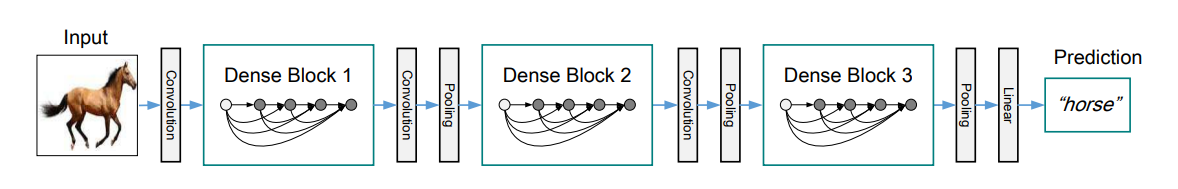
\includegraphics[width=\linewidth]{readings_figures/DenseNet_net.png}
	\caption{DenseNet结构示意图}
	\label{fig:DenseNet_net}
\end{figure}

假设一张图片$x_0$在卷积网络中传播,网络有L层,每一层都实现了非线性转换函数$H_l$,l表示第l层,$H_l$是包含了BN、ReLU、池化和卷积的组合操作,在DenseNet中,$H_l$是BN、ReLU和$3\times3$卷积操作的组合,第l层的输入用$x_l$表示。

那么在传统的神经网络中,将l-1层的输出$x_{l-1}$作为第l层的输入,得到第l层的输出$x_l$,可表示为$x_l=H_l(x_{l-1})$。在ResNet中,添加了skip-connection,可表示为$x_l=H_l(x_{l-1})+x_{l-1}$。在DenseNet中,则采用密集连接的方式,第l层将前面所有层的特征图$[x_0,x_1,x_2,...,x_{l-1}]$作为输入,可表示为$x_l=H_l([x_0,x_1,x_2,...,x_{l-1}])$。

\begin{figure}[htbp]
	\centering
	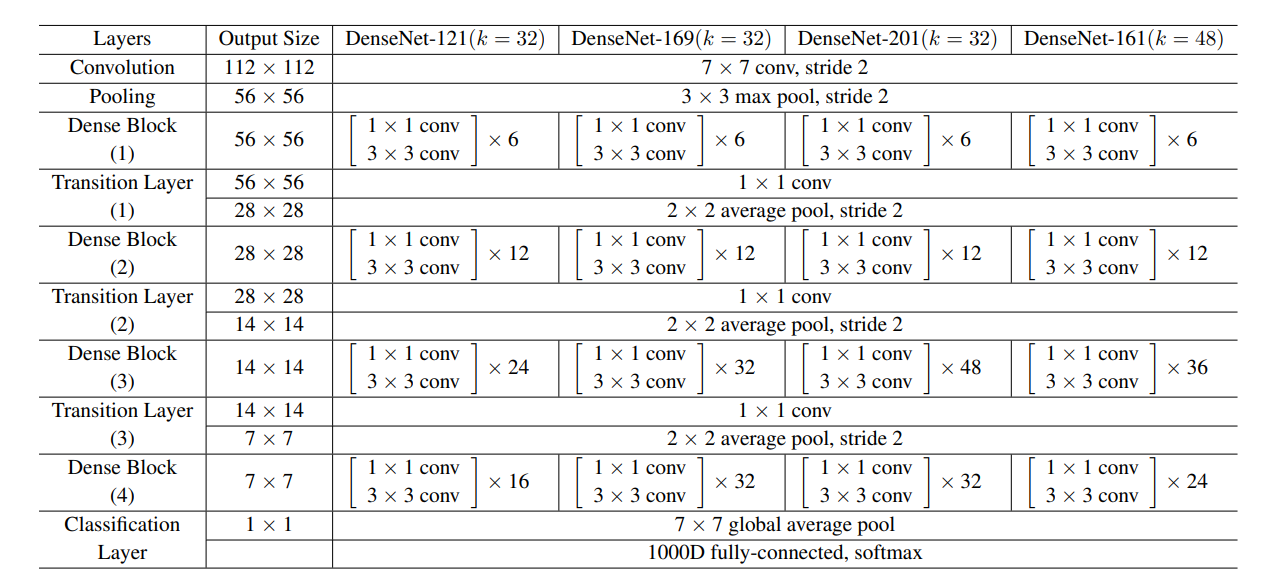
\includegraphics[width=\linewidth]{readings_figures/DenseNet_params.png}
	\caption{DenseNet网络配置}
	\label{fig:DenseNet_params}
\end{figure}

DenseNet在ImageNet数据集上的配置~\ref{fig:DenseNet_params}所示,其中含有:

增长速率k(Growth rate),函数$H_l$产生k个特征图,那么第l层有$k_0+k\times(l-1)$个输入特征图,$k_0$表示输入层的通道数,k就被称为增长速率,控制着每一层能有多少信息对整体网络的状态产生影响,实验证明较小的增长速率就能取得很好的效果。

Bottleneck layers,在$3\times3$卷积层前面加上$1\times1$卷积,可以减少输入的特征图数量,并提高计算效率。

Compression,如果一个dense block包含有m个特征图,那么就让之后的过渡层($1\times1$卷积层后接$2\times2$平均池化层)生成$\theta_m$个输出特征图,$0<\theta\leq1$被称为压缩系数。

\section{SENet}

hu等人\cite{hu2018squeeze}于2017年中提出的SENet获得了2017年的ImageNet挑战赛冠军。作者以另外一种方式思考现有的卷积神经网络实现方式,设计一种新型的结构取得了很好的效果。

传统的卷积神经网络是通过考虑增加网络深度或者宽度的方式从空间维度的角度以提升网络性能,而作者等人从特征通道的角度提出了SENet,关键步骤是squeeze和excitation操作,采用自适应的方式对不同特征通道表达的信息进行学习,对有用的特征进行提升以便更好的训练,而抑制那些没有用或者用处不大的特征。SE模块示意图如~\ref{fig:SENet_SE_module}所示,对于一个输入特征通道数为$c_1$的输入x,经过一系列操作之后特征通道数为$c_2$。对于任意的一组变换$F_{tr}:X \rightarrow U, X \in \mathbb{R}^{W^\prime \times H^\prime \times C^\prime}, U \in \mathbb{R}^{W \times H \times C}$,可以是卷积或者一组卷积,之后构造一组SE模块来完成特征重新校准的操作。特征U首先经过squeeze操作在空间维度上对一个$W \times H$的二维矩阵完成聚合特征映射产生特征通道描述符。该描述符能够表示特征通道响应的全局分布,使较低层能够获得网络全局感受野。之后excitation操作为每个特征通道分配一定的权重。然后特征U被重新加权作为SE模块的输出。

\begin{figure}[htbp!]
	\centering
	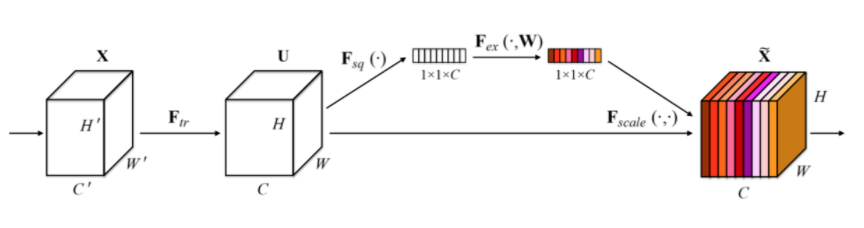
\includegraphics[width=\linewidth]{readings_figures/Squeeze_and_Excitation_module.png}
	\caption{SE模块示意图}
	\label{fig:SENet_SE_module}
\end{figure}

squeeze操作,从空间维度的方面来进行特征压缩,将每一个二维的特征通道转换成一个实数,通过使用全局平均池化生成通道描述符。$z \in \mathbb{R}^C$是对特征U在空间维度$W \times H$上进行收缩形成的,那么z中的第c个元素的计算形式为:

\begin{displaymath}
	z_c = F_{sq}(U_c) = \frac{1}{W \times H}\sum_{i=1}^{W}\sum_{j=1}^{H}u_c(i, j)
\end{displaymath}

excitation操作,采用了简单的类似于循环神经网络中的门机制,并使用sigmoid函数激活:

\begin{displaymath}
	s = F_{ex}(z, W) = \sigma(g(z, W)) = \sigma(W_2 \delta (W_1z))
\end{displaymath}

$\delta$表示ReLU激活函数,降维层参数$W_1 \in \mathbb{R}^{\frac{C}{r} \times C}$,降维比例是r,一般设置为16,升维层参数$W_2 \in \mathbb{R}^{C \times \frac{C}{r}}$。SE模块的最终输出通过重新调节带有激活的变换输出U得到:

\begin{displaymath}
	\tilde{X}_c = F_{scale}(U_c, s_c) = s_c \cdot U_c
\end{displaymath}

$\tilde{X}=[\tilde{x}_1, \tilde{x}_2,\dots, \tilde{x}_C]$和$F_scale(U_c, s_c)$指的是特诊映射$U_c \in \mathbb{R}^{W \times H}$和标量$s_c$之间的对应通道乘积。

SE模块具有优秀的灵活性,可以嵌入到流行的网络架构如Inception和ResNet系列中,将$F_{tr}$看作一个Inception模块,可以构建一个SE-Inception网络~\ref{fig:SE-Inception}:

\begin{figure}[htbp!]
	\centering
	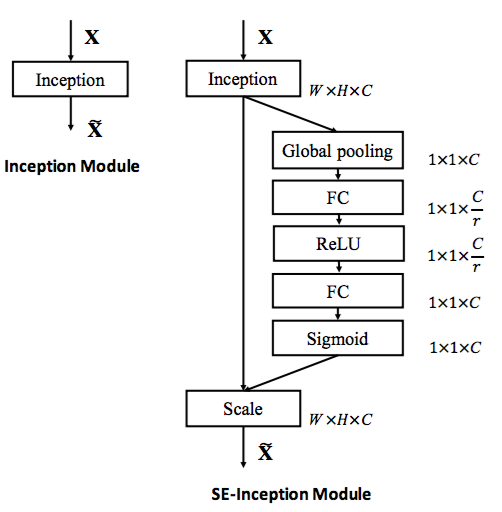
\includegraphics[width=0.5\linewidth]{readings_figures/SE_Inception_module.png}
	\caption{SE-Inception示意图}
	\label{fig:SE-Inception}
\end{figure}

采用全局池化作为squeeze操作,之后采用两个全连接层先降维再进行升维操作,这比单独使用一个全连接层具有了更多的非线性关系,可以更好的拟合通道间复杂的相关性,同时在很大程度上减少了参数量和计算量。之后采用sigmoid激活函数获得0-1之间归一化的权重,最后通过Scale操作将归一化的权重加权到每个通道的特征上。

此外,SE模块还可以嵌入到使用skip-connections的网络中,构建SE-ResNet网络~\ref{fig:SE-ResNet},过程和SE-Inception基本一致。

\begin{figure}[htbp!]
	\centering
	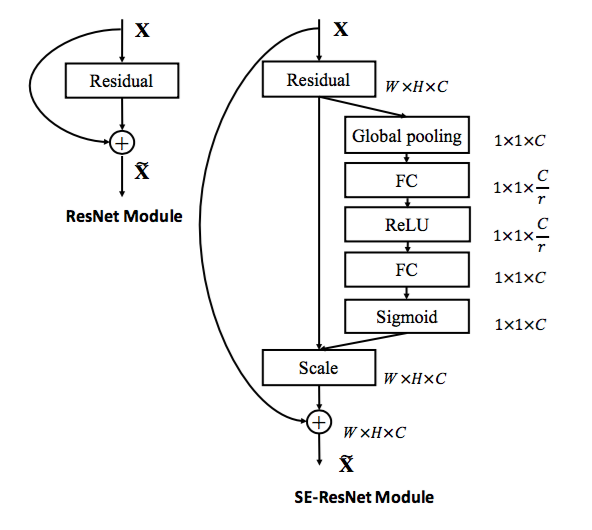
\includegraphics[width=0.5\linewidth]{readings_figures/SE_ResNet_module.png}
	\caption{SE-ResNet示意图}
	\label{fig:SE-ResNet}
\end{figure}



%%----------- 结尾部分 ----------- %%
\clearpage
\phantomsection
\addcontentsline{toc}{chapter}{参考文献}
\bibliography{ref/refs}   % 参考文献
\end{document}
